\section{Metodologia}

A pesquisa possui caráter aplicado, com abordagem quantitativa e objetivo
experimental, e foi conduzida em duas fases (Figura~\ref{fig:fases}). O MVP1 é um
estudo em lote sobre a base NSL-KDD, que compara algoritmos supervisionados e o
efeito da redução de dimensionalidade. O MVP2 é um sistema operacional em tempo
real, cujo desenho responde às limitações observadas no MVP1. Todo o código foi
escrito em Python, com \en{scikit-learn} \cite{Pedregosa2011Scikit, scikit2026learn},
\en{pandas} e \en{scapy}/\en{nfstream} para leitura de pacotes, e o MVP2 é
empacotado em contêineres \en{Docker} \cite{Merkel2014Docker}.

\begin{figure}[H]
  \centering
  % Visão geral das duas fases do trabalho (coluna simples)
\resizebox{\columnwidth}{!}{%
\begin{tikzpicture}[
  node distance=0.35cm and 0.45cm,
  every node/.style={font=\scriptsize},
  block/.style={rectangle, draw, rounded corners=1pt, text width=1.75cm,
                align=center, minimum height=0.85cm, inner sep=2pt},
  fase/.style={draw=azulFEI, dashed, rounded corners=3pt, inner sep=5pt},
  rot/.style={font=\scriptsize\bfseries\sffamily, text=azulFEI},
  arrow/.style={-{Stealth[length=4pt]}}
]
  % MVP1
  \node (nsl)   [block] {Base NSL-KDD};
  \node (pre)   [block, right=of nsl] {Pré-processa\-mento};
  \node (red)   [block, right=of pre] {Correlação, PCA e importância};
  \node (alg)   [block, right=of red] {5 algoritmos supervisio\-nados};
  \node (av)    [block, right=of alg] {Validação + KDDTest+};

  \foreach \a/\b in {nsl/pre, pre/red, red/alg, alg/av} \draw[arrow] (\a) -- (\b);

  % MVP2
  \node (pcap)  [block, below=1.25cm of nsl] {Tráfego espelhado (pcap)};
  \node (feat)  [block, right=of pcap] {17 atributos por fluxo};
  \node (e1)    [block, right=of feat] {Estágio 1: \en{Isolation Forest} + árvore};
  \node (e2)    [block, right=of e1] {Estágio 2: SVM linear};
  \node (an)    [block, right=of e2] {Analista: veredito};

  \foreach \a/\b in {pcap/feat, feat/e1, e1/e2, e2/an} \draw[arrow] (\a) -- (\b);
  \draw[arrow] (an.south) -- ++(0,-0.3) -| node[pos=0.25, below]{rótulos} (e2.south);

  \coordinate (anbaixo) at ([yshift=-0.45cm]an.south);
  \begin{scope}[on background layer]
    \node[fase, fit=(nsl)(av)] (f1) {};
    \node[fase, fit=(pcap)(an)(anbaixo)] (f2) {};
  \end{scope}
  \node[rot, anchor=south west] at (f1.north west) {MVP1 --- estudo em lote};
  \node[rot, anchor=south west] at (f2.north west) {MVP2 --- operação em tempo real};

  \path (f2.north) coordinate (f2topo);
  \draw[arrow, gray, dashed] (av.south) -- (av.south |- f2topo)
     node[midway, right, text width=2.1cm, align=left] {lacuna de generalização};
\end{tikzpicture}%
}

  \caption{Visão geral das duas fases do trabalho.}
  \label{fig:fases}
\end{figure}

% =============================================================================
\subsection{MVP1: Base de Dados e Pré-processamento}

A base utilizada foi a NSL-KDD \cite{Tavallaee2009Detailed}, versão aprimorada da
KDD Cup 1999 que remove registros redundantes e inconsistentes. Os arquivos foram
obtidos pela plataforma \en{Kaggle}\footnote{Disponível em:
\url{https://www.kaggle.com/datasets/hassan06/nslkdd}} com a biblioteca
\en{KaggleHub}. O treino usa o arquivo \cod{KDDTrain+} (125.973 registros) e o
teste final usa o \cod{KDDTest+} (22.544 registros), distribuídos separadamente
pelos autores da base.

Como os arquivos não possuem cabeçalho, os nomes dos 41 atributos foram definidos
manualmente. A coluna \cod{difficulty} foi removida por não descrever o tráfego, e
os atributos \cod{hot} e \cod{logged\_in} também foram descartados. Os atributos
categóricos \cod{protocol\_type} (\cod{tcp}, \cod{udp}, \cod{icmp}),
\cod{service} e \cod{flag} (11 valores) foram analisados e, nos testes que os
utilizam, convertidos por \en{Label Encoding}. Para a comparação principal foram
usados apenas os 36 atributos numéricos restantes.

O rótulo foi tratado de duas formas. Para a análise exploratória, os 22 tipos de
ataque foram agrupados nas categorias clássicas \cite{Belavagi2016Performance,
Jabez2015Intrusion} --- DoS, \en{Probe}, R2L e U2R --- conforme a
Tabela~\ref{tab:categorias}. Para a classificação, o rótulo foi binarizado em
normal (0) ou ataque (1). O conjunto de treino é razoavelmente balanceado nessa
forma: 67.343 registros normais (53,46\%) e 58.630 ataques (46,54\%). As
categorias, porém, são muito desbalanceadas (Figura~\ref{fig:distribuicao}): U2R
tem apenas 52 registros.

\begin{table}[H]
\centering
\footnotesize
\setlength{\tabcolsep}{3pt}
\begin{tabularx}{\columnwidth}{l X r}
\toprule
\textbf{Categoria} & \textbf{Ataques no treino} & \textbf{Registros} \\
\midrule
normal & --- & 67.343 \\
DoS    & neptune, smurf, back, teardrop, pod, land & 45.927 \\
Probe  & satan, ipsweep, portsweep, nmap & 11.656 \\
R2L    & warezclient, guess\_passwd, warezmaster, imap, ftp\_write, multihop, phf, spy & 995 \\
U2R    & buffer\_overflow, rootkit, loadmodule, perl & 52 \\
\bottomrule
\end{tabularx}
\caption{Agrupamento dos ataques do \cod{KDDTrain+} por categoria.}
\label{tab:categorias}
\end{table}

\begin{figure}[H]
  \centering
  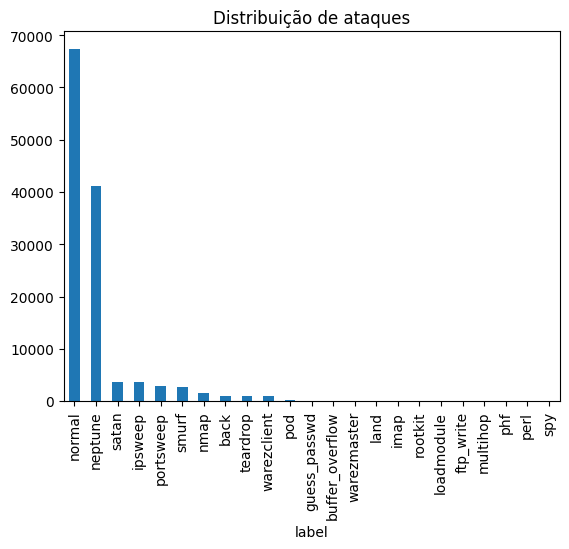
\includegraphics[width=\columnwidth]{distribuicao_ataques.png}
  \caption{Distribuição dos rótulos originais no \cod{KDDTrain+}.}
  \label{fig:distribuicao}
\end{figure}

% =============================================================================
\subsection{MVP1: Redução de Dimensionalidade}

Três técnicas complementares foram aplicadas. Primeiro, a matriz de correlação de
\en{Pearson} entre os atributos numéricos e o rótulo binário, para identificar
redundância e os atributos mais associados a ataques. Segundo, a Análise de
Componentes Principais (PCA), precedida de padronização por \en{StandardScaler}
(média zero e desvio padrão um), já que o PCA é sensível à escala; foi medido o
número de componentes necessários para reter 95\% da variância e gerada uma
projeção em duas dimensões para inspeção visual. Terceiro, a seleção por
importância: uma \en{Decision Tree} foi ajustada sobre os dados padronizados, os
atributos foram ordenados por importância (redução de impureza de Gini) e a mesma
árvore foi retreinada com os $k$ atributos mais importantes, para
$k = 5, \dots, 38$, registrando a acurácia de cada configuração.

% =============================================================================
\subsection{MVP1: Treinamento e Avaliação}

Cinco algoritmos foram comparados, todos com \cod{random\_state = 42}
(Tabela~\ref{tab:algoritmos}). O \cod{KDDTrain+} foi dividido em 80\% para treino
e 20\% para validação, de forma estratificada pelo rótulo. Foram medidas
acurácia, precisão, \en{recall}, \en{F1-score} e os tempos de treino e de predição,
estes últimos relevantes porque o objetivo final é a operação em tempo real.

O melhor modelo da validação foi então retreinado sobre todo o \cod{KDDTrain+} e
avaliado no \cod{KDDTest+}. Essa segunda avaliação é a mais importante do MVP1: o
\cod{KDDTest+} contém tipos de ataque que não existem no treino, o que aproxima o
teste da situação real de um IDS diante de ataques novos.

\begin{table}[H]
\centering
\footnotesize
\renewcommand{\arraystretch}{1.05}
\setlength{\tabcolsep}{2pt}
\begin{tabularx}{\linewidth}{
>{\hsize=0.7\hsize}X
>{\hsize=1.15\hsize}X
>{\hsize=1.15\hsize}X}
\toprule
\textbf{Algoritmo} & \textbf{Definição} \cite{IBM2026Supervised} & \textbf{Motivação} \\
\midrule
\en{Decision Tree} & Regras lógicas em fluxograma que dividem os dados. & Interpretável, baixo custo de predição. \\
\addlinespace
\en{Random Forest} & Combina várias árvores por votação. & Robusto e preciso, porém mais custoso. \\
\addlinespace
KNN ($k=5$) & Classifica pelos vizinhos mais próximos. & \en{Baseline} não paramétrico. \\
\addlinespace
\en{Logistic Regression} & Estima a probabilidade da classe. & \en{Baseline} linear, rápido. \\
\addlinespace
SVM (linear) & Hiperplano de máxima margem. & Eficaz em alta dimensão, lento em lote. \\
\bottomrule
\end{tabularx}
\caption{Algoritmos supervisionados avaliados no MVP1.}
\label{tab:algoritmos}
\end{table}

% =============================================================================
\subsection{MVP2: Arquitetura Geral}

O MVP2 é um NIDS que observa uma cópia passiva do tráfego e classifica cada fluxo
em uma cascata de dois modelos (Figura~\ref{fig:arquitetura}). O Estágio 1 é não
supervisionado porque não existe rótulo no tráfego de produção; ele funciona como
peneira, com \en{recall} alto e precisão baixa. O Estágio 2 é supervisionado e
opera apenas sobre os alertas do Estágio 1, com dois objetivos: recuperar formas
de ataque conhecidas que o Estágio 1 não enxerga e separar ataque real de anomalia
benigna. Os rótulos do Estágio 2 vêm do \en{golden set} e dos vereditos do analista.

\begin{figure*}[t]
  \centering
  \resizebox{\textwidth}{!}{% Arquitetura do MVP2 (largura total da página).
% Três faixas: detecção (cima), ciclo de vida do Estágio 1 (meio),
% refinamento supervisionado (baixo).
\begin{tikzpicture}[
  every node/.style={font=\scriptsize},
  proc/.style={rectangle, draw, rounded corners=2pt, fill=azulFEI!8,
               text width=2.5cm, align=center, minimum height=1.0cm, inner sep=2pt},
  dado/.style={cylinder, shape border rotate=90, aspect=0.18, draw, fill=gray!10,
               text width=2.4cm, align=center, minimum height=1.0cm, inner sep=1pt},
  ator/.style={rectangle, draw, thick, text width=2.3cm, align=center,
               minimum height=0.9cm, inner sep=2pt},
  zona/.style={draw=gray, dashed, rounded corners=4pt, inner sep=7pt},
  rot/.style={font=\scriptsize\sffamily\bfseries, text=gray},
  arrow/.style={-{Stealth[length=4pt]}},
  lbl/.style={font=\tiny, fill=white, inner sep=1pt}
]
  % ---------------- faixa 1: detecção em tempo real (y = 0)
  \node (span)   [ator] at (0,0)    {Porta espelho (SPAN) ou \en{bridge}};
  \node (det)    [proc] at (3.4,0)  {\cod{netanomaly\_live}\\extração de fluxos\\(janela de 10 s)};
  \node (e1)     [proc] at (6.8,0)  {\textbf{Estágio 1}\\\en{Isolation Forest}\\+ árvore \en{surrogate}};
  \node (sink)   [proc] at (10.2,0) {\cod{sink.py}\\percentil contra a grade do treino};
  \node (alerts) [dado] at (13.6,0) {\cod{na.alerts}\\(\en{hypertable})};

  % ---------------- faixa 2: ciclo de vida do Estágio 1 (y = -2.9)
  \node (pool)   [dado] at (10.2,-2.9) {\en{Pool} de \en{parquets} + \cod{feature\_windows}};
  \node (cand)   [proc] at (6.8,-2.9)  {\cod{lifecycle}\\\cod{candidate}\\(diário, automático)};
  \node (gate)   [proc] at (3.4,-2.9)  {Portão por cenário\\(\cod{v\_gate\_verdict})};
  \node (prom)   [ator] at (0,-2.9)    {Promoção manual\\(troca atômica)};
  \node (gold)   [dado] at (3.4,-4.5)  {\en{Golden set}\\(cenários rotulados)};

  % ---------------- faixa 3: refinamento supervisionado (y = -6.6)
  \node (e2)     [proc] at (13.6,-6.6) {\textbf{Estágio 2}\\SVM linear\\(\cod{netclassify})};
  \node (fila)   [dado] at (10.2,-6.6) {Predições e fila por margem};
  \node (ana)    [ator] at (6.8,-6.6)  {Analista\\(painel Grafana)};
  \node (ver)    [dado] at (3.4,-6.6)  {\cod{na.verdicts}};
  \node (final)  [dado] at (0,-6.6)    {Classificação final consolidada};

  % setas: detecção
  \draw[arrow] (span) -- (det);
  \draw[arrow] (det) -- (e1);
  \draw[arrow] (e1) -- node[lbl, above=2pt]{escore} (sink);
  \draw[arrow] (sink) -- node[lbl, above=2pt]{$p \geq 0{,}95$} (alerts);

  % setas: ciclo de vida
  \draw[arrow] (sink) -- node[lbl, right=2pt, align=left]{janelas de\\13 min} (pool);
  \draw[arrow] (pool) -- node[lbl, below=3pt, align=center]{quarentena 7 d\\meia-vida 14 d} (cand);
  \draw[arrow] (cand) -- (gate);
  \draw[arrow] (gold) -- (gate);
  \draw[arrow] (gate) -- node[lbl, above=2pt]{aprovado} (prom);
  \draw[arrow] (prom.north) -- ++(0,0.75) -| node[lbl, pos=0.3, above]{novo \texttt{current\_flow.joblib}} (e1.south);

  % setas: refinamento
  \draw[arrow] (alerts) -- node[lbl, right=2pt]{alertas} (e2);
  \draw[arrow] (e2) -- (fila);
  \draw[arrow] (fila) -- node[lbl, above=2pt]{menor margem} (ana);
  \draw[arrow] (ana) -- node[lbl, above=2pt]{veredito} (ver);
  \draw[arrow] (ver.south) -- ++(0,-0.55) -| node[lbl, pos=0.25, below]{rótulos para retreino} (e2.south);
  \draw[arrow] (ver) -- (final);
  \draw[arrow] (fila.north) -- ++(0,0.55) -| node[lbl, pos=0.25, above]{predição (sem veredito)} (final.north);

  \begin{scope}[on background layer]
    \node[zona, fit=(span)(alerts)] (z1) {};
    \node[zona, fit=(prom)(pool)(gold)] (z2) {};
    \node[zona, fit=(final)(e2)] (z3) {};
  \end{scope}
  \node[rot, anchor=south east] at (z1.north east) {detecção em tempo real};
  \node[rot, anchor=south east] at (z2.south east) {ciclo de vida do Estágio 1};
  \node[rot, anchor=north west] at (z3.south west) {refinamento supervisionado};
\end{tikzpicture}
}
  \caption{Arquitetura do MVP2: detecção em tempo real, refinamento supervisionado e ciclo de vida do modelo do Estágio 1.}
  \label{fig:arquitetura}
\end{figure*}

Os componentes de \en{software} são:
\begin{itemize}
  \item \cod{netanomaly.py}: extração de atributos, treino do Estágio 1, métricas e
  rotulagem do CIC-IDS-2017 pelo cronograma oficial;
  \item \cod{netanomaly\_live.py}: analisador em tempo real, que aplica o modelo
  congelado a janelas de 10 s;
  \item \cod{sink.py}: persistência, que grava janelas no \en{pool} de treino e
  alertas no banco;
  \item \cod{lifecycle.py}: ciclo de vida do Estágio 1 (\en{pool}, candidato,
  portão, promoção, despejo, adoção);
  \item \cod{netclassify.py}: Estágio 2 (veredito, treino, avaliação, promoção,
  predição e fila de revisão);
  \item \cod{migrations/}: esquema PostgreSQL/TimescaleDB, versionado por migração.
\end{itemize}

% =============================================================================
\subsection{MVP2: Extração de Atributos}

Os atributos do NSL-KDD não podem ser reproduzidos a partir de um \en{pcap}
arbitrário: vários dependem de inspeção de conteúdo e de contadores internos do
sensor original. Por isso o MVP2 define seu próprio vetor, calculável diretamente
dos cabeçalhos dos pacotes. O MVP1 contribuiu com a ordem de grandeza (17
atributos) e com a evidência de que volume, contagem e taxa de erro de conexão são
os sinais mais discriminantes. Duas visões são suportadas
(Tabela~\ref{tab:atributos}): por fluxo, agregando a 5-tupla bidirecional, e por
\en{host}, agregando por IP de origem para capturar o leque de conexões
(\en{fan-out}) típico de varreduras. A visão por fluxo foi a exercitada de ponta a
ponta.

\begin{table}[H]
\centering
\footnotesize
\setlength{\tabcolsep}{3pt}
\begin{tabularx}{\columnwidth}{l X}
\toprule
\textbf{Grupo} & \textbf{Atributos} \\
\midrule
\multicolumn{2}{l}{\textit{Visão por fluxo (17)}} \\
Volume      & \cod{n\_packets}, \cod{n\_bytes}, \cod{duration}, \cod{bytes\_per\_sec}, \cod{pkts\_per\_sec} \\
Tamanho     & \cod{mean\_len}, \cod{std\_len}, \cod{min\_len}, \cod{max\_len} \\
Tempo       & \cod{mean\_iat}, \cod{std\_iat} (intervalo entre pacotes) \\
Flags TCP   & \cod{syn\_ratio}, \cod{ack\_ratio}, \cod{fin\_ratio}, \cod{rst\_ratio}, \cod{psh\_ratio}, \cod{syn\_no\_ack} \\
\midrule
\multicolumn{2}{l}{\textit{Visão por host de origem (11)}} \\
Leque       & \cod{n\_dst}, \cod{n\_dports}, \cod{dports\_per\_dst}, \cod{pkts\_per\_dst} \\
Volume      & \cod{h\_packets}, \cod{h\_bytes}, \cod{h\_pkts\_per\_sec} \\
Handshake   & \cod{h\_syn\_ratio}, \cod{h\_ack\_ratio}, \cod{h\_rst\_ratio}, \cod{syn\_ack\_gap} \\
\bottomrule
\end{tabularx}
\caption{Vetores de atributos do MVP2.}
\label{tab:atributos}
\end{table}

% =============================================================================
\subsection{MVP2: Estágio 1 --- Detector e Explicação}

O detector é um \cod{StandardScaler} seguido de um \cod{IsolationForest} com 200
árvores, ambos ajustados com pesos por amostra iguais ao peso de recência da
janela de origem (Seção~III-H). O escore é invertido para que valores maiores
signifiquem mais anomalia, e o limiar $\tau$ é o quantil \emph{ponderado} do
escore de treino:

\begin{equation}
  s(x) = -\,\mathrm{score}(x), \qquad
  \tau = Q_w\!\left(1 - c\right),
  \label{eq:limiar}
\end{equation}

\noindent em que $c$ é o \en{contamination} e $Q_w$ é o quantil calculado sobre a
distribuição acumulada ponderada pelos pesos $w$. Usar o quantil simples com
pesos no ajuste faria o limiar responder a amostras que o modelo praticamente
ignorou. O limiar é \emph{congelado} no artefato: o analisador ao vivo nunca o
recalcula, pois isso faria a taxa de alerta depender da composição da janela
corrente e não do treino.

Junto ao limiar, o artefato guarda uma grade de 1.001 quantis do escore de treino.
O percentil de cada fluxo é calculado contra essa grade, e não contra os demais
fluxos da mesma janela. Percentil relativo à janela produziria alerta por
construção: em uma janela sem ataque algum, o “1\% mais anômalo” é tráfego
normal. Contra a grade do treino, uma janela tranquila não gera alerta, e o
percentil fica disponível imediatamente, sem esperar a janela fechar.

Para a explicabilidade, uma \cod{DecisionTreeClassifier} de profundidade 4 é
treinada sobre os atributos \emph{não escalados}, tendo como alvo o rótulo
atribuído pelo próprio \en{Isolation Forest}. A regra do caminho percorrido por
cada alerta (por exemplo, \cod{n\_dports > 50 e duration <= 2,1}) é exibida ao
analista em unidades reconhecíveis. A árvore explica, mas não decide.

% =============================================================================
\subsection{MVP2: Estágio 2 --- Refinador Supervisionado}

O Estágio 2 usa \cod{StandardScaler} e \cod{LinearSVC} com $C=1$ e
\cod{class\_weight="balanced"}, porque ataque é a classe minoritária. Os
atributos de entrada são os 17 do fluxo; o escore do Estágio 1 está
disponível em cada alerta para versões futuras. O SVM linear foi escolhido, em vez
de uma clusterização pura, porque sua \cod{decision\_function} fornece a
distância com sinal ao hiperplano, usada para priorizar a revisão. A clusterização
fica reservada como apoio à rotulagem em lote.

\textbf{Partida a frio.} Uma instalação nova não tem nenhum veredito. O primeiro
hiperplano é treinado sobre o \en{golden set} (capturas rotuladas como ataque ou
benigno) e entra em produção com a decisão registrada como \emph{adotado}, pois não
passou por portão. Os vereditos do analista são somados ao treino à medida que
chegam e valem como rótulo da rede real.

\textbf{Operação.} O comando \cod{predict} aplica o SVM promovido a cada alerta e
grava a classe predita, o valor de decisão e a margem. A fila de revisão é
ordenada por margem crescente: os casos mais próximos da fronteira aparecem
primeiro, que é onde o veredito mais move o hiperplano (aprendizado ativo por
incerteza \cite{Settles2009Active}). Para o painel, uma projeção PCA em duas
dimensões é ajustada no treino e congelada no artefato, de modo que pontos de
janelas diferentes sejam comparáveis.

\textbf{Anotar, não suprimir.} O Estágio 2 reordena e anota a fila, mas não
descarta alerta automaticamente. Supressão automática criaria falso negativo
silencioso justamente quando o modelo, recém-treinado com poucos vereditos, ainda
erra mais. A classificação final consolidada segue a precedência
\emph{veredito $>$ Estágio 2 $>$ apenas Estágio 1 (pendente)}.

\textbf{Vereditos.} Cada veredito guarda uma cópia do vetor de atributos, porque a
retenção de alertas é de 180 dias e o rótulo precisa sobreviver ao alerta que o
originou. Revisões não sobrescrevem: criam uma nova linha que aponta para a
anterior, preservando divergências entre analistas como informação.

% =============================================================================
\subsection{MVP2: Ciclo de Vida e Defesa contra Envenenamento}

A decisão central do ciclo de vida é que o detector \textbf{nunca é retreinado na
janela de tráfego mais recente}. O \en{Isolation Forest} aprende como normal a
massa dos dados que recebe; se a janela contém ataque, o ataque passa a ser normal
e deixa de ser marcado. Isso é explorável de forma gradual: um canal de comando e
controle (C2) com batida de 6~h é absorvido um pouco mais a cada retreino, sem que
o atacante precise evadir nada \cite{Biggio2012Poisoning}. O que o dado recente
compra de fato é redução de falso positivo (servidor novo, mudança de horário de
\en{backup}). Por isso o treino ocorre sobre um \en{pool} curado
(Figura~\ref{fig:ciclo}):

\begin{itemize}
  \item \textbf{Janela de \en{pool}:} o \cod{sink} agrupa os fluxos em janelas de
  780 s (13 min), alinhadas da mesma forma para captura ao vivo e para
  \en{pcap} histórico. É uma cadência distinta da janela de análise de 10 s, que
  só determina a latência do alerta.
  \item \textbf{Quarentena:} a janela só entra no \en{pool} depois de 7 dias sem
  indicador de comprometimento (IOC) retroativo.
  \item \textbf{Recência:} cada janela recebe peso
  $w = 0{,}5^{\,(t_{\max}-t)/h}$, com meia-vida $h = 14$ dias, normalizado pela
  janela mais nova do \en{pool} --- sem a normalização, uma captura histórica teria
  peso da ordem de $10^{-64}$. Janelas com $w < 0{,}05$ são descartadas. A
  amostragem (limitada a 2 milhões de linhas) é proporcional ao tamanho da janela e
  serve só para limitar memória; a recência entra apenas pelo \cod{sample\_weight},
  para não ser aplicada duas vezes.
  \item \textbf{Despejo e procedência:} cada modelo registra quais janelas o
  treinaram. Descoberto um comprometimento, as janelas do período são despejadas,
  a consulta \cod{v\_models\_contaminados} lista os modelos que as absorveram e um
  novo candidato é treinado sem elas --- algo impossível em aprendizado incremental.
  \item \textbf{Homogeneidade:} janelas com contratos de atributos diferentes não
  são misturadas, pois isso geraria um modelo cujo vetor de entrada não existe.
\end{itemize}

\begin{figure}[H]
  \centering
  % Estados de uma janela de tráfego e os três relógios do ciclo de vida
\resizebox{\columnwidth}{!}{%
\begin{tikzpicture}[
  node distance=0.45cm and 0.55cm,
  every node/.style={font=\scriptsize},
  est/.style={rectangle, draw, rounded corners=6pt, fill=azulFEI!8,
              text width=1.6cm, align=center, minimum height=0.8cm, inner sep=2pt},
  mau/.style={est, fill=red!10},
  arrow/.style={-{Stealth[length=4pt]}},
  lbl/.style={font=\tiny, align=center}
]
  \node (jan)  [est] {Janela capturada (13 min)};
  \node (qua)  [est, right=of jan] {Quarentena};
  \node (ati)  [est, right=of qua] {\en{Pool} ativo};
  \node (pes)  [est, right=of ati] {Peso $\to$ 0 (cauda)};
  \node (des)  [mau, below=0.9cm of ati] {Despejada};
  \node (mod)  [mau, right=of des] {Modelos contaminados};

  \draw[arrow] (jan) -- (qua);
  \draw[arrow] (qua) -- node[lbl, above]{7 dias sem\\IOC} (ati);
  \draw[arrow] (ati) -- node[lbl, above]{$w<0{,}05$} (pes);
  \draw[arrow] (qua.south) |- node[lbl, pos=0.3, left]{IOC\\retroativo} (des.west);
  \draw[arrow] (ati) -- node[lbl, right]{IOC} (des);
  \draw[arrow] (des) -- node[lbl, above]{procedência} (mod);
\end{tikzpicture}%
}

  \caption{Estados de uma janela de tráfego no \en{pool} de treino.}
  \label{fig:ciclo}
\end{figure}

O ciclo é regido por três relógios separados: a árvore \en{surrogate} é
atualizada a cada janela; um candidato é treinado e medido diariamente, de forma
automática; e a promoção para produção é semanal ou sob demanda e
\textbf{sempre manual}. Um portão que se auto-aprova não é portão: com poucos
cenários no \en{golden set}, ele daria aparência de verificação ao que não foi
verificado. Ao promover, o modelo anterior e as árvores que o descreviam são
aposentados e o artefato é trocado por \cod{rename()} atômico de um \en{symlink},
que o detector recarrega sem reinício. O analista também pode pedir retreino
manual, mas o pedido registra junto o número de quase-acertos que o justifica ---
alertas confirmados como ataque que ficaram abaixo do corte, medidos pela consulta
\cod{v\_stage1\_near\_misses}.

% =============================================================================
\subsection{MVP2: Golden Set e Portão de Promoção}

O \en{golden set} é um conjunto de capturas rotuladas, organizado por cenário
(Tabela~\ref{tab:cenarios}). As capturas podem ser registradas manualmente, a
partir de testes de intrusão feitos pelo próprio operador, ou derivadas do
cronograma oficial de ataques do CIC-IDS-2017 \cite{Sharafaldin2018Toward}.
Todo candidato é avaliado por captura, por cenário e no agregado.

\begin{table}[H]
\centering
\footnotesize
\setlength{\tabcolsep}{3pt}
\begin{tabularx}{\columnwidth}{l X c c}
\toprule
\textbf{Cenário} & \textbf{Descrição} & \textbf{E1} & \textbf{E2} \\
\midrule
recon        & Varredura de portas e \en{hosts} (nmap) & 0,90$^*$ & 0,90 \\
brute\_force & Força bruta em SSH, FTP, HTTP & --- & 0,85 \\
exfil        & Exfiltração por canal incomum & --- & 0,80 \\
beacon\_1h   & C2 com batida horária & --- & 0,75 \\
beacon\_6h   & C2 com batida de 6~h & --- & 0,60 \\
lateral      & Movimento lateral (SMB, RDP) & --- & 0,80 \\
benigno      & Controle limpo: mede falso positivo & FPR & FPR \\
\bottomrule
\end{tabularx}
\caption{Cenários do \en{golden set} e piso de \en{recall} exigido por estágio. $^*$não obrigatório até haver captura real.}
\label{tab:cenarios}
\end{table}

Um candidato é reprovado se \emph{qualquer} cenário isolado: (i) cair mais de
0,10 de \en{recall} em relação ao modelo em produção; (ii) ficar abaixo do piso
absoluto do cenário; ou (iii) exceder 2\% de falso positivo no controle benigno. O
terceiro critério impede que um candidato degenerado, que alerta em tudo, passe
com \en{recall} 1,00 em todos os cenários. A avaliação é por cenário, e não
agregada, porque o envenenamento lento aparece como a queda de \emph{um} cenário
específico, que a média esconde.

Os pisos são definidos por estágio. O \en{Isolation Forest} é estruturalmente
cego a ataques volumosos e homogêneos (Seção~IV-D); exigir \cod{brute\_force} dele
tornaria o portão do Estágio 1 impossível de passar. Assim, o Estágio 1 é cobrado
de varredura e falso positivo, e os ataques densos são cobrados do Estágio 2.

\textbf{Adoção.} Uma instalação nova enfrenta um impasse circular: o detector
precisa de modelo promovido, a promoção precisa de candidato, o candidato precisa
de \en{pool}, e o \en{pool} é alimentado pelo detector. O comando \cod{adopt} rompe o
círculo com um modelo treinado fora do ciclo: valida o contrato de atributos, gera
a grade de percentis a partir da captura de treino, semeia o \en{pool} com essa
captura (registrando a procedência) e registra o modelo como \emph{adotado}. O
detector, por sua vez, não treina sozinho: em uma instância vazia ele aguarda,
explicando o que falta, pois treinar no tráfego que estiver passando é exatamente
o caminho do envenenamento.

% =============================================================================
\subsection{MVP2: Persistência}

O banco é PostgreSQL 17 com a extensão TimescaleDB, organizado no esquema
\cod{na} (14 tabelas e 11 consultas, \en{views}, após as migrações). Quatro
decisões estruturam o esquema:

\begin{enumerate}
  \item \textbf{Fluxos não vão para o banco.} Uma captura de 10~GB gera milhões de
  fluxos; o treino quer formato colunar comprimido. Os fluxos ficam em arquivos
  \en{Parquet} em disco, e o banco guarda um índice deles (\cod{feature\_windows}),
  com estado de quarentena e despejo. Só o que vira alerta entra como linha.
  \item \textbf{O corte do analista é aplicado na consulta.} Há dois limiares: o
  piso de gravação (percentil 0,95, fixo) e o corte de exibição (0,99, ajustável).
  Como o corte é aplicado em uma \en{view}, alterá-lo tem efeito retroativo sem
  reprocessar nada.
  \item \textbf{Escore e percentil são guardados juntos.} O percentil permite ao
  analista raciocinar em porcentagem; o escore contínuo alimenta o Estágio 2.
  \item \textbf{Sem chave estrangeira para alertas.} A tabela de alertas é uma
  \en{hypertable} com retenção de 180 dias; vereditos e predições referenciam o
  alerta com integridade garantida pela aplicação.
\end{enumerate}

Os parâmetros operacionais (limiares, quarentena, meia-vida, tolerâncias do
portão) ficam em uma tabela editável com histórico de alterações por gatilho. As
migrações são aplicadas uma única vez cada por um controlador próprio, cada uma em
transação junto com seu registro; se uma falha, o contêiner aborta de propósito.

% =============================================================================
\subsection{MVP2: Implantação em Contêineres}

Uma única imagem (\cod{python:3.13-slim}) serve aos papéis de detector, treinador
e utilitários, garantindo a mesma versão de \en{scikit-learn} em todos --- requisito,
pois o artefato \cod{.joblib} é serializado por versão. Nenhum contêiner roda como
\en{root}: as capacidades \cod{cap\_net\_raw} e \cod{cap\_net\_admin} são
atribuídas ao binário \cod{tcpdump} como \en{file capabilities}, de modo que um
processo de UID 1000 abre o \en{socket} de captura. A Tabela~\ref{tab:servicos}
resume os serviços do \en{Docker Compose}.

\begin{table}[H]
\centering
\footnotesize
\setlength{\tabcolsep}{3pt}
\begin{tabularx}{\columnwidth}{l l X}
\toprule
\textbf{Serviço} & \textbf{Perfil} & \textbf{Função} \\
\midrule
banco            & ---              & TimescaleDB, porta só em \cod{127.0.0.1} \\
treinador        & ---              & Migrações e relógio diário de candidatos \\
detector         & sensor           & Captura em \cod{network\_mode: host} \\
detector-isolado & sensor-isolado   & NIC dedicada via \en{macvlan passthru} \\
replay           & replay           & Reprocessa um \en{pcap}, sem captura \\
grafana          & painel           & Painéis dos Estágios 1, 2 e resultado final \\
\bottomrule
\end{tabularx}
\caption{Serviços do \en{Docker Compose} e perfis de ativação.}
\label{tab:servicos}
\end{table}

Um contêiner só enxerga o tráfego que chega ao seu \en{namespace} de rede. Por
isso o \en{macvlan} em modo \en{bridge}, opção mais intuitiva, não serve para IDS:
o \en{kernel} entrega ao contêiner apenas o tráfego destinado ao seu próprio
endereço MAC. As opções válidas são o modo \en{host}, que vê uma interface
promíscua ligada à porta espelho (SPAN) do \en{switch}, e o \en{macvlan
passthru}, que entrega a placa inteira ao contêiner. O arranjo recomendado usa
duas interfaces: uma de gerência, com IP, e uma de captura, sem IP e em modo
promíscuo. No laboratório, a máquina virtual do sensor roda sobre Proxmox, com a
interface em modo promíscuo e a \en{bridge} virtual com \en{ageing time} zero, o
que faz a \en{bridge} repassar todos os quadros a todas as portas, à maneira de
um \en{hub}.

Os painéis do Grafana leem diretamente o banco e cobrem: o Estágio 1 (alertas
acima do corte, quase-acertos, janelas no \en{pool}, portão do último candidato);
o Estágio 2 (dispersão do SVM em PCA 2D, desempenho por cenário, fila por margem);
e o resultado final consolidado, com a classificação ao longo do tempo e o acerto
contra o rótulo real quando disponível. A arquitetura prevista para o
\en{front-end} é híbrida: parâmetros editados por um painel de formulários do
próprio Grafana, e a tela de veredito como aplicação própria na mesma origem,
via \en{proxy} reverso, evitando desligar a sanitização de HTML do Grafana.

% =============================================================================
\subsection{MVP2: Protocolo de Avaliação}

Duas fontes de dados foram usadas, com papéis distintos:

\begin{itemize}
  \item \textbf{CIC-IDS-2017} \cite{Sharafaldin2018Toward}: capturas reais
  (\en{pcap}) rotuladas pelo cronograma oficial dos ataques, com tratamento de
  NAT. O ataque FTP-Patator, da terça-feira, foi usado como \en{golden set} real de
  \cod{brute\_force}.
  \item \textbf{Gerador sintético} (\cod{scripts/gerar\_sintetico.py}): produz
  \en{pools} e capturas de varredura, beacon e tráfego normal com distribuições
  controladas. Os números obtidos com ele medem o \emph{mecanismo} (portão,
  quarentena, despejo), nunca a capacidade real de detecção.
\end{itemize}

As métricas principais são o \en{recall} por cenário e a taxa de falso positivo
(FPR) no controle benigno; ROC-AUC e precisão média (AP) complementam a análise do
Estágio 1. Os experimentos de envenenamento usam 5 sementes aleatórias, com o
gerador re-semeado antes de cada \en{pool}, porque seu estado compartilhado faria a
composição do \en{pool} depender da ordem das chamadas. Por fim, uma demonstração de
ponta a ponta (\cod{scripts/demo\_ataque.sh}) sobe um atacante e uma vítima em
contêineres, executa uma varredura \cod{nmap} e verifica se o pipeline grava
alertas usando o mesmo modelo, banco e código da produção.
